\begin{activity} \label{A:10.7.10} While the quantity of a product
  demanded by consumers is often a function of the price of the
  product, the demand for a product may also depend on the price of
  other products.  For instance, the demand for blue jeans at Old Navy may be affected not only by the price of the jeans themselves, but also by the price of khakis.

  Suppose we have two goods whose respective prices are $p_1$ and
  $p_2$.  The demand for these goods, $q_1$ and $q_2$, depend on the
  prices as 
  \begin{align}
    q_1 &= 150 - 2p_1 - p_2 \label{eq:good1} \\
    q_2 &= 200 - p_1 - 3p_2. \label{eq:good2}
  \end{align}

  The seller would like to
  set the prices $p_1$ and $p_2$ in order to maximize revenue. 
  We will assume that the seller meets the full demand for each product. Thus, if we let $R$ be the revenue obtained by
  selling $q_1$ items of the first good at price $p_1$ per item and $q_2$
  items of the second good at price $p_2$ per item, we have
  \[R = p_1q_1 + p_2q_2.\] 
  We can then write the
  revenue as a function of just the two variables $p_1$ and $p_2$ by using Equations
  (\ref{eq:good1}) and (\ref{eq:good2}), giving us
  \[R(p_1,p_2) = p_1(150 - 2p_1 - p_2) + p_2(200 - p_1 - 3p_2)= 150p_1
  + 200p_2 - 2p_1p_2 -2p_1^2 - 3p_2^2.\] A graph of $R$ as a function
  of $p_1$ and $p_2$ is shown in Figure \ref{F:10.7.Optimize1}.
  \begin{figure}[h]
    \begin{center}
      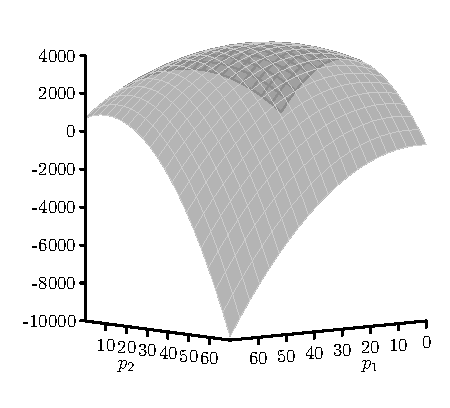
\includegraphics{figures/fig_10_7_revenue.eps}
    \end{center}
    \caption{A revenue function.}
    \label{F:10.7.Optimize1}
  \end{figure}
  \ba
  \item Find all critical points of the revenue function, $R(p_1, p_2)$.
  \item Apply the Second Derivative Test to determine the type of any
    critical points.
  \item Where should the seller set the prices $p_1$ and $p_2$ to maximize the
    revenue? 

\ea
\end{activity} 

\begin{activitySolution}
\ba 
\item To find the critical points we determine where $R_{p_1}$ and $R_{p_2}$ are simultaneously 0 (since $R$ is a polynomial function, the partial derivatives of $R$ exist everywhere).  Now
\[R_{p_1}(p_1,p_2) = 150 - 2p_2 - 4p_1 \ \ \text{ and } \ \ R_{p_2}(p_1,p_2) = 200 - 2p_1 - 6p_2.\]
The system
\begin{align*}
R_{p_1}(p_1,p_2) &= 0 \\
R_{p_2}(p_1,p_2) &= 0
\end{align*}
or
\begin{align*}
150 - 2p_2 - 4p_1 &= 0 \\
200 - 2p_1 - 6p_2 &= 0
\end{align*}
is a system of two linear equations in two unknowns. Multiplying both sides of the second equation by $-2$ and then adding corresponding sides of this new equation with the first equation yields the equation
\[-250 + 10p_2 = 0\]
or
\[p_2 = 25.\]
Substituting back into the first equation shows that
\[p_1 = 25.\]
Thus, our only critical point occurs at $(25, 25)$. 

\item To apply the second derivative test, we need the second order partial derivatives:
\[R_{p_1p_1}(p_1,p_2) = -4, \ \ R_{p_1p_2}(p_1,p_2) = -2, \ \ R_{p_2p_2}(p_2,p_2) = -6.\]
So the discriminant of $R$ at the critical point $(25,25)$ is 
\[D = R_{p_1p_1}(25,25) R_{p_2p_2}(25,25) - R_{p_1p_2}(25,25)^2 = 24-4=20 > 0,\]
and $R$ has a relative maximum at the critical point. the graph of $R$ indicates an absolute maximum as well at the critical point, so the price for each item should be set at 25 dollars to maximize the revenue. Note that the maximum revenue is $R(25,25) = 4375$. 

\ea
\end{activitySolution}

\aftera 